\let\negmedspace\undefined
\let\negthickspace\undefined
\documentclass[journal]{IEEEtran}
\usepackage[a5paper, margin=10mm, onecolumn]{geometry}
%\usepackage{lmodern} 
\usepackage{tfrupee} 

\setlength{\headheight}{1cm} 
\setlength{\headsep}{0mm}     

\usepackage{gvv-book}
\usepackage{gvv}
\usepackage{cite}
\usepackage{amsmath,amssymb,amsfonts,amsthm}
\usepackage{algorithmic}
\usepackage{graphicx}
\usepackage{textcomp}
\usepackage{xcolor}
\usepackage{txfonts}
\usepackage{listings}
\usepackage{enumitem}
\usepackage{mathtools}
\usepackage{gensymb}
\usepackage{comment}
\usepackage[breaklinks=true]{hyperref}
\usepackage{tkz-euclide} 
\usepackage{listings}                                        
\def\inputGnumericTable{}                                 
\usepackage[latin1]{inputenc}                                
\usepackage{color}                                            
\usepackage{array}                                            
\usepackage{longtable}                                       
\usepackage{calc}                                             
\usepackage{multirow}                                         
\usepackage{hhline}                                           
\usepackage{ifthen}                                           
\usepackage{lscape}

\begin{document}

\bibliographystyle{IEEEtran}
\vspace{3cm}

\title{9.8.5}
\author{AI25BTECH11003 - Bhavesh Gaikwad}
{\let\newpage\relax\maketitle}

\renewcommand{\thefigure}{\theenumi}
\renewcommand{\thetable}{\theenumi}
\setlength{\intextsep}{10pt} 


\numberwithin{equation}{enumi}
\numberwithin{figure}{enumi}
\renewcommand{\thetable}{\theenumi}


\textbf{Question}: Let $\vec{S}$ be the focus of the parabola $y^2 = 8x$ and let PQ be the common chord of the circle $x^2 + y^2 - 2x - 4y = 0$ and the given parabola. The area of the triangle PQS is\\\\

\textbf{Solution:}\\
  Given:\\
$\quad \text{Circle: }x^2 + y^2 - 2x - 4y = 0$\\
$\text{Parabola: }y^2 = 8x$\\\\


Parameters of the Circle:
\begin{equation}
\vec{V}_1 = \myvec{1 & 0 \\ 0 & 1}, \, \vec{u}_1 = \myvec{-1 \\ -2}, \, f_1 = 0   
\end{equation}

Parameters of the Parabola:
\begin{equation}
\vec{V}_2 = \myvec{0 & 0 \\ 0 & 1}, \, \vec{u}_2 = \myvec{-4 \\ 0}, \, f_2 = 0, \, \vec{S} = \myvec{2e \\ 0 } = \myvec{2 \\ 0}   
\end{equation}

Points of Intersection of Circle and Parabola can be given as:
\begin{equation}
\vec{X}^\top(\vec{V}_1+\mu\vec{V}_2)\vec{X} + 2(\vec{u}_1+\mu\vec{u}_2)^\top\vec{X} + (f_1 + \mu f_2) = 0
\end{equation}

\begin{equation}
\vec{X}^\top\myvec{1 & 0 \\ 0 & 1+\mu}\vec{X} - 2\myvec{1+4\mu & 2}\vec{X} = 0    
\end{equation}


\begin{equation}
\text{To degenerate a conic into a line, we can find values of $\mu$ by} \norm{\vec{M}_1 + \mu\vec{M}_2} =0
\end{equation}
where $\vec{M}_i = \myvec{\vec{V}_i & \vec{u}_i \\ \vec{u}_i^\top & f_i}$\\

From Equation 0.5, we get 
\begin{equation}
    (4\mu+1)^2(\mu + 1) = -4
\end{equation}

\begin{equation}
\Rightarrow \, \, \mu = \dfrac{-5}{4} \text{ (as the only real solution.)}    
\end{equation}

Substituting the value of $\mu$ in Equation 0.4,
\begin{equation}
\vec{X}^\top\myvec{1 & 0 \\ 0 & -1/4}\vec{X} + \myvec{8 & -4}\vec{X} = 0
\end{equation}

\begin{equation}
    (2x+y+16)(2x-y) = 0
\end{equation}

\begin{equation}
   \Rightarrow \, \, 2x + y + 16 =0 \text{ OR } 2x-y=0
\end{equation}

From Line $2x + y + 16 =0$, we get no points of intersection with both the conics.\\
Thus, Rejected this Case.\\

From Line $2x-y=0$
\begin{equation}
    \vec{X} = k\myvec{2 \\ -1} 
\end{equation}

The Intersection of the given conic with the given line can be written as:
\begin{equation}
    \vec{x}_j = \vec{h} + k_j\vec{m}
\end{equation}

\begin{equation}
where, \, \vec{h} = \myvec{0 \\ 0} \, \& \, \vec{m} = \myvec{2 \\ -1}   
\end{equation}

\begin{equation}
    k_{j} = \left( \dfrac{1}{\vec{m}^\top\vec{V}_i\vec{m}} \right) \left( 
    -\vec{m}^\top(\vec{V}_i\vec{h}+\vec{u}_i) \, \pm \, \sqrt{[\vec{m}^\top(\vec{V}_i\vec{h}+\vec{u}_i)]^2 - g(h)(\vec{m}^\top\vec{V}_i\vec{m})} \right) 
\end{equation}

After Solving the Equation 0.12 with circle and parabola, We get common points of intersection as:
\begin{equation}
    \vec{X}_1 = \myvec{0 \\ 0} \qquad \& \qquad \vec{X}_2 = \myvec{2 \\ 4}
\end{equation}

Therefore,
Let $\vec{P} = \myvec{0 \\ 0}$ and $\vec{Q} = \myvec{2 \\ 4}$\\\\

The Area of Triangle PQS is:
\begin{equation}
    Area(\triangle PQS) = \dfrac{1}{2}\norm{\vec{SP} \times \vec{QP}} = 4
\end{equation}

\begin{align*}
    \boxed{\text{The Area of $\triangle PQS$ is 4 sq.units.}}
\end{align*}


\begin{figure}[htbp]
    \centering
    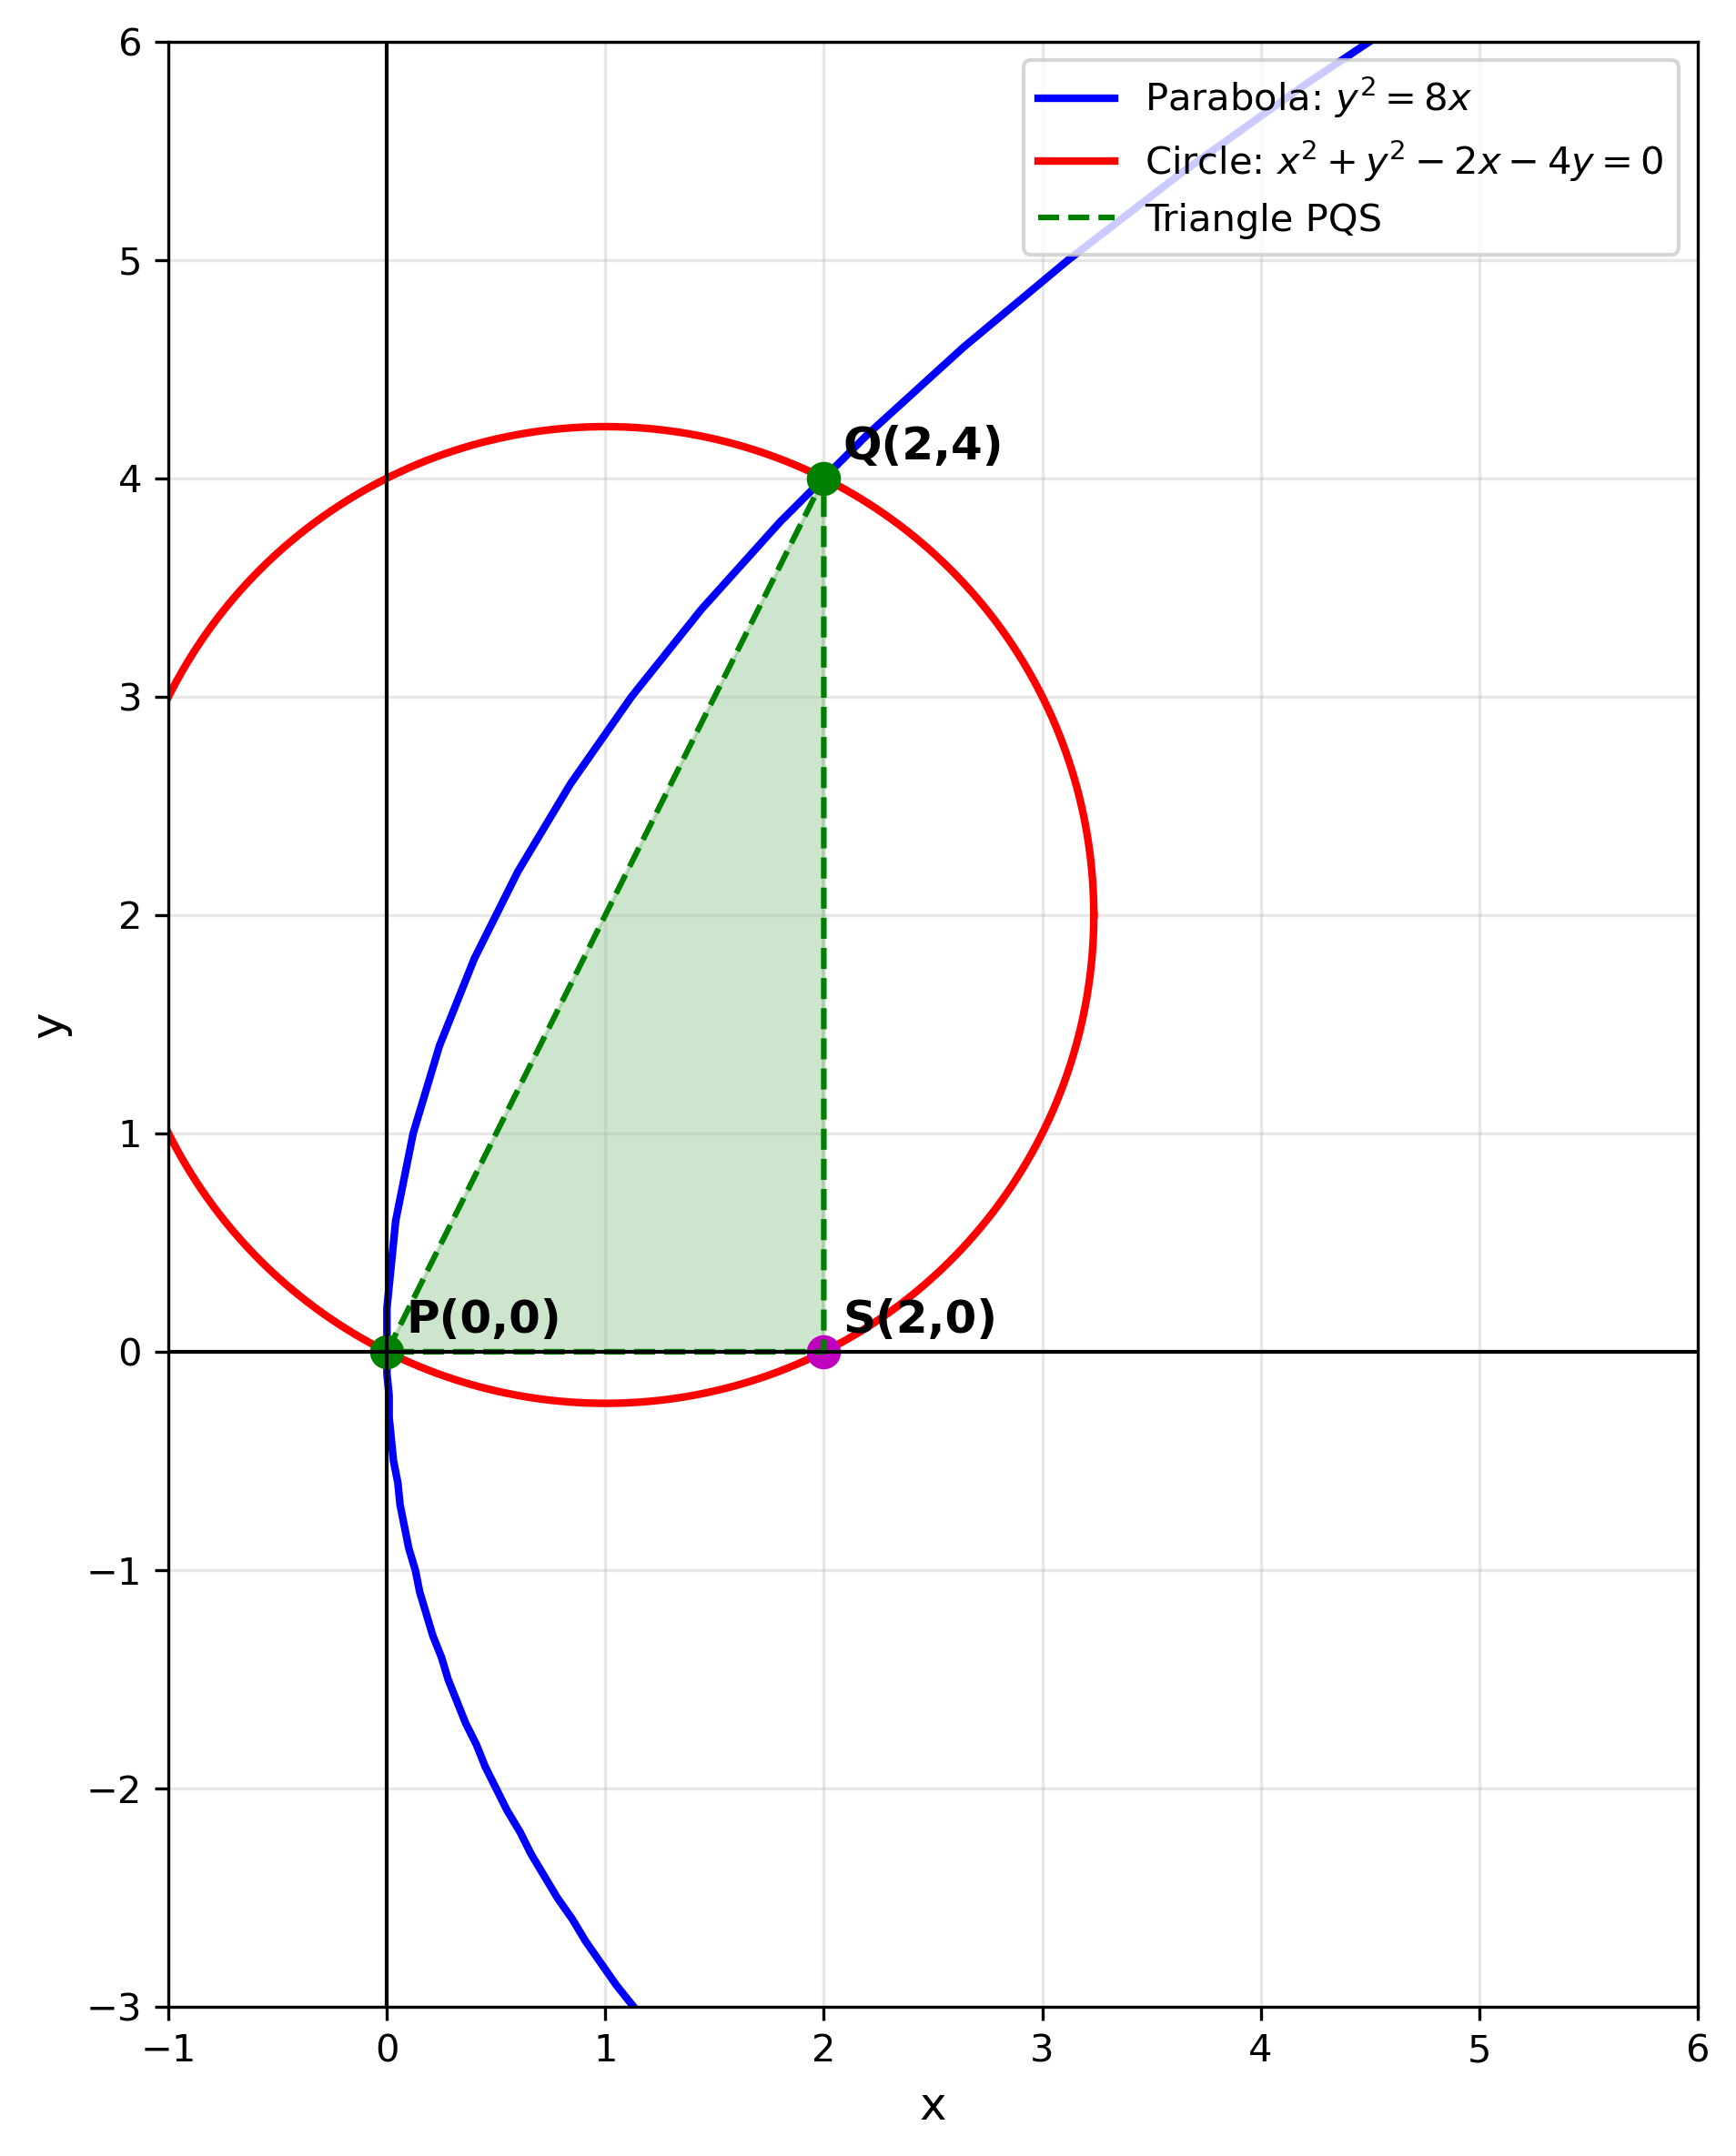
\includegraphics[width=0.9\columnwidth]{figs/fig1.png}
    \caption{Intersection of Two Conics and Triangle PQS}
    \label{fig:figs/fig1.png}
\end{figure}

\end{document}  
